\documentclass{report}
\usepackage[spanish]{babel}
\usepackage{graphicx}
\usepackage{mathtools}

\begin{document}

\tableofcontents

\chapter{Conceptos introductorios}

\section{Algunas definiciones importantes}
{\footnotesize Créditos a Alfonso por el capitulo 1, 2 y 3}
\begin{itemize}
	\item Economía: La economía es el estudio del modo en que la sociedad gestiona sus recursos escasos. La escasez significa que la sociedad tiene unos recursos limitados y, por lo tanto, no puede producir todos los bienes y servicios que los individuos desean tener.

	\item Escasez: Carácter limitado de los recursos limitados de una sociedad.

	\item Eficiencia: Significa que la sociedad aprovecha de la mejor manera posible los recursos escasos.

	\item Equidad: Significa que la prosperidad económica se distribuye equitativamente entre los miembros de la sociedad.

	\item Microeconomía: La microeconomía es la parte de la economía que estudia las partes individuales de la economía (como los hogares y las empresas interactúan, y cómo interactúan con los mercados).

	\item Macroeconomía: La macroeconomía es una parte de la economía que ve a la economía como un todo.

	\item Mercado: Un ámbito físico o no en el que interactúan oferentes y demandantes en el que se negocia el intercambio de dinero por bienes. El mercado es un grupo de compradores y vendedores de un bien o de un servicio

	\item Nivel de vida: Refiere a la accesibilidad de los individuos de una sociedad a los diferentes bienes y servicios esenciales y no esenciales.

	\item Déficit fiscal: describe la situación en la cual los gastos (como asistencia social y salarios) realizados por el Estado superan a los ingresos no financieros (como lo son el pago de impuestos y multas), en un determinado período.

	\item Bien Normal: Aquel bien cuya demanda disminuye al disminuir la renta (ingreso) del consumidor.

	\item Bien Inferior: Aquel bien cuya demanda aumenta al disminuir la renta del consumidor.

	\item Ley de demanda: La cantidad demandada de un bien está relacionada negativamente (inversamente) con el precio de dicho bien.

	\item Ley de oferta: La cantidad ofrecida de un bien está relacionada positivamente (directamente) con el precio de dicho bien.

	\item Equilibrio: Situación en la que la oferta y la demanda se equilibran.

	\item Inflación: es un aumento sostenido del nivel general de precios de la economía

	\item Ceteris paribus: Este término se utiliza por los economistas para indicar que todas las variables pertinentes, salvo las que están estudiando en ese momento, se mantienen constantes.

	\item INE: Instituto Nacional de Estadística. Liniers 1280 (Atrás de la torre ejecutiva).

	\item BCU: Banco Central del Uruguay. Diagonal fabini.
\end{itemize}

\chapter{10 principios de la economia}

\section{Principios 1 - 4: ¿Cómo toman decisiones los individuos}
\subsection{Principio de la disyuntiva}
Este principio establece que cuando se agrupan individuos en sociedades, estos se enfrentan a disyuntivas (toma de decisiones o TradeOffs) que afectan el modo en que invierten sus recursos para así obtener uno u otro beneficio a cambio. Una disyuntiva importante a la que se enfrenta la sociedad es la de la eficiencia y la equidad. La eficiencia refiere a intentar sacar el mayor provecho a los recursos escasos con los que cuenta dicha sociedad, mientras que la equidad a la forma de distribuír los beneficios y aquellos recursos entre la sociedad de manera equitativa.

Ej: Un ejemplo es el caso de un estudiante que ha de decidir cómo va a repartir su tiempo (recurso). Puede dedicarlo todo a estudiar economía o todo a estudiar psicología, o puede repartirlo entre las dos materias.  Por cada hora que estudia una de ellas, está renunciando a una hora que podría estar dedicando a la otra. Y por cada hora de estudio, tienen una hora menos para dedicar a las actividades extracurriculares.

\subsection{Principio del coste de oportunidad}
Cuando los individuos se enfrentan a una disyuntiva, deben comparar coste-beneficio de las diferentes posibilidades. Sin embargo, muchas veces este contraste no es tan evidente. El coste de oportunidad de una cosa es aquello a lo que renunciamos para conseguirla.
Ej: Los deportistas en edad universitaria que pueden ganar millones si abandonan los estudios y juegan deportes profesionales son muy conscientes de que para ellos el coste de oportunidad de los estudios universitarios es muy alto.

\subsection{Principio del pensamiento marginal}
Los economistas utilizan el término cambios marginales para referirse a los pequeños ajustes que uno realiza a la hora de tomar acción en un plan que ya existe. No todo debe ser blanco o negro, sino que existen ciertos matices de grises.
Se dice que una persona toma una decisión racional si y sólo si el beneficio marginal es superior al coste marginal; y utiliza el pensamiento racional para tomar decisiones comparando costos y beneficios marginales.
Ej: Nosotros tenemos planeado un día productivo de estudio, llevamos 3 horas adquiriendo conocimientos pero nos empezamos a cansar. Aquí se presenta una pequeña disyuntiva; seguimos estudiando o nos vamos a descansar. Frente a esto tendremos que comparar un coste marginal contra un beneficio marginal; aprender un poco más o dejar por acá e ir a dormir.

\subsection{Principio de los incentivos}
Como la toma de decisiones se hace comparando coste-beneficio, muchas veces la conducta de un individuo puede cambiar si cambian estos costes o beneficios. En otras palabras, los individuos responden a los incentivos. Sin embargo, el implementar un incentivo para cambiar la conducta de los individuos puede traer consigo consecuencias colaterales imprevistas.
Ej: Por ejemplo, un impuesto sobre la gasolina anima a la gente a utilizar automóviles más pequeños, que consumen menos gasolina. También la anima a utilizar el transporte público en lugar del automóvil y a vivir más cerca del centro de trabajo. Si el impuesto es suficientemente alto, comenzará a utilizar automóviles eléctricos.


\section{Principios 5 - 7: ¿Cómo interactúan los individuos?}
\subsection{El comercio puede mejorar el bienestar de todo el mundo}
En la economía, que dos sociedades compitan no significa que una gane o pierda en una interacción, sino todo lo contrario, el comercio entre dos países mejora el bienestar de los dos.
La competencia económica implica que una sociedad (y sus individuos) pueda especializarse en aquello que mejor hace y disfrutar de bienes y servicios mayor, muchas veces provenientes de la competencia. Dentro del comercio, competidor y socio pueden ser lo mismo.

\subsection{Los mercados normalmente constituyen un buen mecanismo para organizar la actividad económica}
Una economía de mercado es un tipo de economía que asigna recursos por medio de las decisiones descentralizadas de muchas empresas y hogares cuando interactúan en mercados de bienes y servicios.
Las empresas son las que deciden a quiénes contratar, qué van a producir, y los hogares y consumidores son los que deciden qué consumir. Los hogares y las empresas interactúan en el mercado, en los cuales los precios y el interés orientan sus decisiones. A pesar de que la toma de decisiones está descentralizada y de que los que toman las decisiones buscan su propio provecho, las economías de mercado han demostrado tener un éxito notable en la organización de la actividad económica de una forma que promueva el bienestar económico general.

\textbf{Adam Smith y la mano invisible}: Los hogares y las empresas interactúan en los mercados como si fueran guiados por una mano invisible que los condujera a obtener unos resultados de mercado deseables. Los precios en un mercado son el instrumento con el que la mano invisible dirige la actividad económica. Por eso, los precios guían a quienes toman las decisiones hacia resultados que maximizan el bienestar de la sociedad en su totalidad. La acción de la mano invisible se ve interrumpida por la participación del gobierno.

\subsection{Fallas de mercado}
Una falla de mercado se refieren a dichas situaciones en las que el mercado no asigna eficientemente los recursos por sí solo por lo que el Estado debe intervenir.
Posibles causas:
Externalidad negativa: Es la consecuencia de la acción de un agente para el bienestar de otro.
Poder monopólico: Sucede cuando una empresa o grupo de individuos logran ser los únicos oferentes de cierto bien o servicio. En ese caso el precio de dicho bien o servicio no está sujeto a las interacciones del mercado, sino al precio que los individuos puedan pagar.
Pobreza: basada en la canasta básica alimentaria (CBA) que pueden comprar.

\section{Principios 8 - 10: ¿Cómo funciona la economía en su conjunto?}
\subsection{Productividad y nivel de vida}
Casi todas las diferencias entre los niveles de vida son atribuidas a las diferencias entre los niveles de productividad de los países, que es la cantidad de bienes y servicios producidos con cada hora de trabajo.
La relación entre la productividad y los niveles de vida tiene profundas implicaciones en la política económica. Para elevar los niveles de vida, los responsables de la política económica tienen que elevar la productividad asegurándose de que los trabajadores tienen un buen nivel de estudios, poseen las herramientas necesarias para producir bienes y servicios y tienen acceso a la mejor tecnología existente.


\subsection{Los precios suben cuando el gobierno imprime demasiado dinero}
La inflación es un aumento sostenido del nivel general de precios de la economía.
El principal causante de este fenómeno es el crecimiento de la cantidad de dinero. Al aumentar la cantidad de dinero que fluye por la sociedad, éste pierde valor, ya que está perdiendo escasez. Entonces las personas que tienen ingresos fijos como jubilados y trabajadores sufren la devaluación de sus salarios. Al ser cada vez un bien más común, el poder adquisitivo del dinero cae lo que produce que los precios se disparen. \\

$$RF = T  - [ G + TR + Ig + Id ]$$
$RF$: Resultado fiscal ( Si es positivo es un Superavit Fiscal, de caso contrario un Deficit FIscal) \\
$T$: Ingreso del Estado (Impuestos) \\
$G$: Gastos del Estado (Sueldos de Funcionarios) \\
$TR$: Transferencias (Jubilaciones) \\
$Ig$: Refacciones o reparaciones de obras públicas \\
$Id$: Intereses por deuda \\

Cuando RF \textless \ 0, decimos que estamos en situación de Déficit fiscal. \\
Caso contrario, hablamos de Superávit fiscal. \\

Fenómeno: ¿Por qué se produce el déficit fiscal? Al entrar en un Déficit Fiscal, el gobierno necesita sacar dinero de algún lado. Aquí recurre al sector privado ofreciendo bonos a un interés dado. Si esto falla y el gobierno genera desconfianza hacia las empresas y manda la señal de producir más dinero al Banco Central, aumentando el flujo de dinero y finalmente generando inflación.

\subsection{Tradeoff a corto plazo entre inflación y desempleo}
La razón predominante por la cual es difícil librarse de la inflación, es que a menudo se piensa que la reducción de la inflación provoca un aumento temporal del desempleo. \\
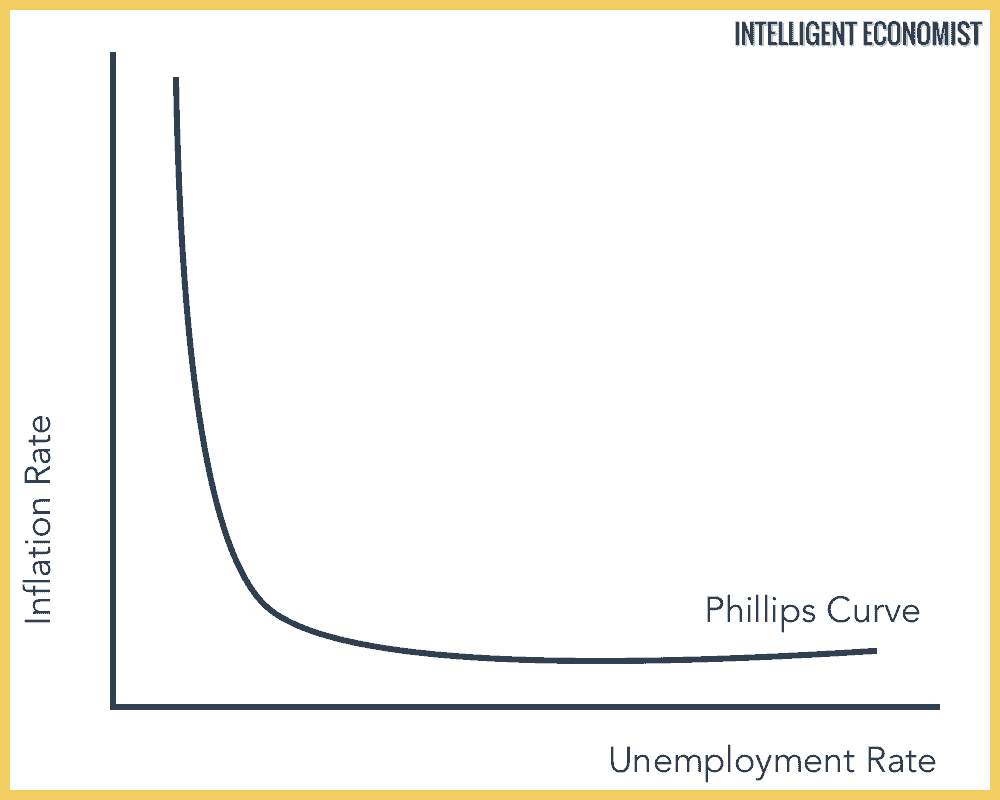
\includegraphics[width=8cm]{../Assets/phillips-curve.png} \\

$\pi$ : Inflación \\

$\mu$: Desempleo \\

Cuando $\pi \uparrow \Rightarrow \mu \downarrow$
Cuando el gobierno reduce, por ejemplo, la cantidad de dinero, reduce la cantidad que gastan los individuos. Una disminución del gasto, junto con unos precios demasiado altos, reduce la cantidad de bienes y servicios que venden las empresas. Una disminución de las ventas lleva, a su vez, a las empresas a despedir trabajadores. Por lo tanto, la reducción de la cantidad de dinero eleva el desempleo temporalmente hasta que los precios se ajusten totalmente en respuesta al cambio.

En la década del 70 se produjo un fenómeno económico muy interesante llamado estanflación en el cual la tasa de desempleo era muy alta produciendo un estancamiento y la tasa de inflación también era alta.

\chapter{Pensar como un economista}

\section{El economista como un científico}
Los economistas enfocan el estudio de forma muy similar a los físicos, elaborando teorías y recogiendo datos y analizar para intentar verificarla o refutarlas. La esencia de la ciencia es el método científico, es decir, el desarrollo y la contrastación desapasionados de teorías sobre el modo en que funciona el mundo.

\textbf{El método científico; observación, teoría y más observación}: El obstáculo al que se enfrentan los economistas es la dificultad para hacer experimentos. Por ello, los economistas prestan especial atención a los experimentos naturales que ofrece la historia. 

\textit{\footnotesize Ej: Cuando estalla una guerra en Oriente Medio que interrumpe el suministro de crudo, los precios del petróleo se disparan en todo el mundo. Para los consumidores de petróleo y de sus derivados, este tipo de acontecimiento reduce su nivel de vida.}

\textbf{El papel de los supuestos}: Los economistas postulan supuestos ya que permiten simplificar la realidad y comprender el mundo de manera más fácil.

\textit{\footnotesize Ej: para estudiar los efectos del comercio internacional, podemos suponer que el mundo está formado únicamente por dos países y que cada uno de ellos solo produce dos bienes. De esta manera es posible centrar el estudio en los aspectos importantes. Una vez comprendido el comercio internacional en una situación tan hipotética, estamos en mejores condiciones para comprenderlo en el mundo más complejo que es la actualidad.}

La cuestión está en saber qué supuestos debemos postular, o, en otras palabras, utilizar supuestos adecuados para estudiar distintas circunstancias. El uso de supuestos facilita muchas cosas, pero hay que tener cuidado y saber cuáles usar antes de trabajar en un hucho en concreto.

\textit{\footnotesize Ej: para estudiar los efectos a corto plazo de la política económica, podemos suponer que los precios no varían mucho. Sin embargo, para estudiar los efectos a largo plazo de la política económica, podemos suponer que todos los precios son absolutamente flexibles.}

\section{Los modelos económicos}

El uso de modelos en cualquier disciplina es muy útil para explicar y trabajar una realidad dada. Los economistas utilizan modelos formados por diagramas y ecuaciones para comprender el mundo, omitiendo detalles para facilitar su comprensión. Es decir que, los modelos económicos no contienen todos los rasgos de la economía.

\subsection{Primer modelo. El diagrama del flujo circular}
Es un modelo visual de la economía que muestra cómo fluyen los dólares por los mercados, entre los hogares y las empresas, siendo estos dos tipos de agentes que toman decisiones (Tradeoffs). \\
Empresas: producen bienes y servicios utilizando factores como lo son el trabajo, la tierra y el capital; denominados factores de producción. \\
Hogares: poseen factores de producción y consumen bienes y servicios brindados por las empresas.

Estos agentes interactúan en dos tipos de mercados.
Mercados de bienes y servicios: los hogares son compradores y las empresas los vendedores de bienes y servicios.
Mercados de factores de producción (trabajo): los hogares son los vendedores y las empresas son compradores de factores que éstas utilizan para producir bienes y servicios.

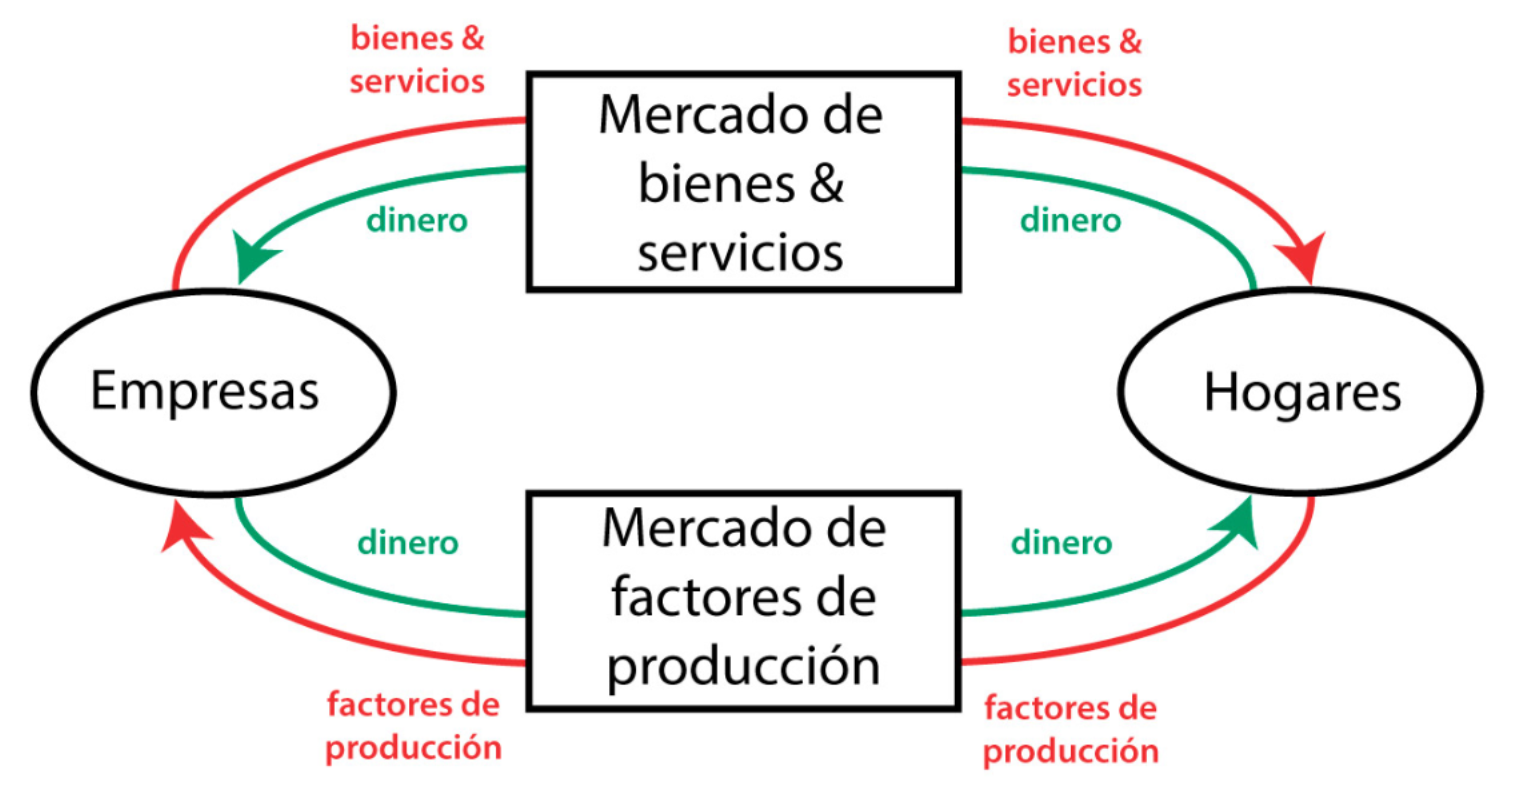
\includegraphics[width=10cm]{../Assets/mercados_economia.png}

{\footnotesize Por lo tanto, lo que ocurre en los diagramas de flujo circular es que los hogares venden su trabajo, tierras y capital a las empresas en los mercados de factores de producción. 
Las empresas utilizan estos factores para producir bienes y servicios, los cuales se venden a su vez a los hogares en los mercados de bienes y servicios. Limitaciones: No considera la intervención del gobierno en la economía. No incorpora el sector financiero. No presenta las relaciones con el resto del mundo.} \\

\subsection{Segundo modelo: La frontera de posibilidades de producción}
Obviamente, la mayoría de las economías producen miles de bienes y servicios. Sin embargo, imaginemos que sólo produjeran dos; un factor productivo \(x\) y otro \(y\). Estas dos industrias juntas utilizan todos los factores de producción de la economía. La frontera de posibilidades de producción de esta economía es un gráfico que muestra todas las diversas combinaciones de productos (\(x\) e \(y\)) que puede producir la economía dados los factores de producción que dispone y la tecnología de producción con la que cuenta: \\

\includegraphics[width=10cm]{../Assets/Frontera_de_posibilidades_de_producción.png} \\

Se dice que un resultado es eficiente si la economía está sacando el mayor provecho posible de los recursos escasos con los que cuenta. Aquellos puntos que se encuentran en la frontera de producción son todos aquellos puntos considerados eficientes. Cuando la economía decide pararse en uno de estos puntos, no puede producir más de uno de los bienes sin sacrificar la producción del otro. En otras palabras, la frontera del gráfico muestra el coste de oportunidad de un bien en función del otro. Por otro lado, el punto B representa un resultado ineficiente.

También podemos ver la curva como la disyuntiva a la que se enfrenta la sociedad a la hora de decidir qué y cuánto producir. Esta disyuntiva puede ir variando con el tiempo, al variar la curva, los recursos necesarios para la producción, el beneficio, etc.

\section{La microeconomía y la macroeconomía}

La economía tradicionalmente se divide en dos grandes campos: \\
\textbf{Microeconomía}: Es el estudio del modo en que los hogares y las empresas toman decisiones, y de la forma en que interactúan en los mercados. \\
\textbf{Macroeconomía}: Es el estudio de los fenómenos que afectan al conjunto de la economía, entre los que se encuentran la inflación, el desempleo y el crecimiento económico.

Como los cambios de la economía global son el resultado de las decisiones de millones de personas, es imposible comprender los fenómenos macroeconómicos sin examinar las decisiones microeconómicas correspondientes. 

Como la microeconomía y la macroeconomía abordan cuestiones diferentes, a veces adoptan enfoques muy distintos y suelen enseñarse en cursos separados.

El economista y su papel en la formulación de la política económica:

A menudo se pide a los economistas que expliquen las causas de los acontecimientos económicos. Cuando los economistas tratan de explicar el mundo, son científicos; y cuando tratan de mejorarlo, formulan la política económica.

\subsection{Análisis positivo y normativo}
Como los científicos y los encargados de formular la política económica tienen diferentes objetivos, utilizan el lenguaje de forma distinta.

Las afirmaciones sobre el mundo son de dos tipos \\
\textbf{Afirmaciones positivas (descriptivo)}: son afirmaciones que intentan describir el mundo tal como es, como. \\
\textbf{Afirmaciones normativas (prescriptivas)}: son afirmaciones que intentan prescribir cómo debería ser el mundo.

Una diferencia clave entre las afirmaciones positivas y las normativas es el modo en que juzgamos su validez. En principio, podemos confirmar o refutar las afirmaciones positivas examinando la evidencia. En cambio, en la evaluación de afirmaciones normativas intervienen tanto valores como hechos. 	Nuestras ideas positivas sobre el modo en que funciona el mundo afectan a nuestras ideas normativas sobre cuáles son las medidas deseables.

\subsection{Por qué discrepan los economistas}
A menudo, se critica a los economistas en su conjunto por dar consejos contradictorios a los responsables de la política económica. Los economistas suelen discrepar sobre la validez de las distintas teorías positivas del modo en que funciona el mundo. Pueden tener valores diferentes y, por lo tanto, puntos de vista normativos diferentes sobre lo que debe tratar de conseguir la política económica.

\textbf{Diferencias entre los juicios científicos}: Los economistas a veces discrepan porque tienen presentimientos diferentes sobre la validez de las distintas teorías o sobre la magnitud de importantes parámetros.

\textit{\footnotesize Ej: Los economistas discrepan sobre la conveniencia de que el gobierno grava la renta de los hogares o su consumo (su gasto). Los que son partidarios de que se sustituya el impuesto actual sobre la renta por un impuesto sobre el consumo creen que este cambio animaría a los hogares a ahorrar más, ya que la renta que se ahorra no estaría sujeta a impuestos.
Un aumento del ahorro aceleraría, a su vez, el crecimiento de la productividad y de los niveles de vida. Los defensores del impuesto actual sobre la renta creen que el ahorro de los hogares no respondería mucho a un cambio de la legislación tributaria. Estos dos grupos de economistas tienen opiniones normativas diferentes sobre el sistema tributario, ya que tienen ideas positivas diferentes sobre la sensibilidad del ahorro a los incentivos fiscales.}

\textbf{Diferencias entre los valores}: Una política económica no puede juzgarse desde un punto de vista exclusivamente científico. Los economistas dan a veces consejos contradictorios porque tienen valores diferentes. 

\textbf{Percepción frente a realidad}: Es inevitable que haya algunas discrepancias entre los economistas, puesto que emiten juicios científicos distintos y tienen valores diferentes. Sin embargo, no debemos exagerar el grado de discrepancia. En muchos casos los economistas ofrecen una opinión unánime. 

{\footnotesize Turismo de no residentes del país o también llamado \textbf{turismo receptor} involucra una importación de dólares del lado de los turistas y una exportación de servicios de parte del país. Recordar que cuando se habla de importación/exportación, no solo se habla de bienes materiales, sino también de servicios.}


\chapter{Microeconomía}

\section{Las fuerzas del mercado}

La oferta y la demanda son dos fuerzas que refieren a la conducta de las personas al interrelacionarse en los mercados, permitiendo que funcionen las economías de mercado. Determina la cantidad producida de cada bien y el precio al que se vende. Si queremos saber cómo afectará a la economía un acontecimiento o una medida económica, debemos pensar primero cómo afecta a la oferta y la demanda.

\section{Tipos de mercado y la competencia}

\textbf{Mercados competitivos}: Es un mercado en el que hay muchos compradores y muchos vendedores, por lo que cada uno de ellos ejerce una influencia insignificante en el precio de mercado. Los vendedores tienen pocas razones para cobrar un precio inferior al vigente, y si cobran más, los compradores acudirán a otros, la competencia.

Los bienes que se ofrecen en venta son todos iguales.\\
Los compradores y los vendedores son tan numerosos que ningún comprador ni ningún vendedor puede influir en el precio de mercado. \\
Vendedores y compradores son “tomadores de precio”. \\

\textbf{Monopolio}: Es un tipo de mercado en el que el vendedor de un bien es único, y este puede fijar el precio de dicho bien. \\

\textbf{Oligopolio}:  Existen unos pocos vendedores que no compiten ferozmente.\\

\textbf{Monopolísticamente competitivo}: Un mercado en el que hay varios vendedores, pero cada uno ofrece un producto algo diferente, por lo que tienen cierta flexibilidad a la hora de fijar precios. \\

Veremos que se demuestra que los mercados competitivos son más eficientes que los monopolios.

\section{Ley de demanda}

\[ P \uparrow ~ \Rightarrow Q_d \downarrow \]

\[
	(D_M): Q_d = Q(\underset{-}{P};\underset{+-}{R};\underset{+}{P^S};\underset{-}{P^C};\underset{-}{G};\underset{+-}{Exp};\underset{+}{N})
\]
\section{Ley de oferta}

\[
	P \uparrow \Rightarrow Q_d \uparrow
\]

\[
	(S_M): Q_s = Q(\underset{+}{P};\underset{-}{P_{ins}};\underset{-}{W};\underset{+}{\tau};\underset{+-}{Exp};\underset{+}{N})
\]

\section{Equilibrio}

\textbf{Equilibrio}: Situación en la que la oferta y la demanda se equilibran. O sea, es el punto en el que la cantidad ofrecida Qs y la cantidad demandada Qd son iguales. Lo mismo sucede con los precios. \\

\textbf{Precio de equilibrio}: precio que equilibra la oferta y la demanda. A este precio todos los agentes del mercado están satisfechos. Gráficamente, es el precio de la intersección de la curva de oferta y demanda. \\

\textbf{Cantidad de equilibrio}: la cantidad demandada y ofrecida al precio de equilibrio. Gráficamente, es la cantidad donde se cortan la curva de oferta y demanda. \\

\section{Cambio de equilibrio}

\textbf{Exceso}: Los oferentes no son capaces de vender todo lo que desean al precio vigente, ya que el precio de mercado es superior al de equilibrio. Por lo tanto, los oferentes deberán bajar el precio para aumentar las ventas, moviéndose nuevamente hacia el equilibrio. \\

\textbf{Escasez}: Los demandantes no pueden comprar toda la oferta al precio vigente, ya que el precio de mercado es inferior al de equilibrio. Por lo tanto, los oferentes aumentarán los precios, moviéndose nuevamente hacia el equilibrio. \\

\section{Ley de oferta y demanda}

Las actividades de los numerosos compradores y vendedores llevan automáticamente al precio de mercado hacia el precio de equilibrio. Este fenómeno se denomina ley de oferta y demanda, que establece que el precio de un bien se ajusta para equilibrar su oferta y su demanda. 
Debido a esto sabemos que la cantidad demandada y la cantidad ofrecida son iguales cuando el precio del mercado es el precio de equilibrio.

\section{Politica economica}

El gobierno puede determinar precios minimos y maximos. Veremos que esto, dependiendo del caso, puede afectar el precio del mercado y la situacion.

\subsection{Precio maximo}
Un maximo legal que es superior al precio de equilibrio no afectara al mercado.
Sin embargo, si el precio maximo es inferior al precio de equilibrio se generara una situacion de escasez.

\subsection{Precio minimo}
Un minimo legal que es inferior al precio de equilibrio no afectara al mercado.
Sin embargo, si el precio minimo es superior al precio de equilibrio se generara una situacion de exceso.

\section{Esquema fotito}

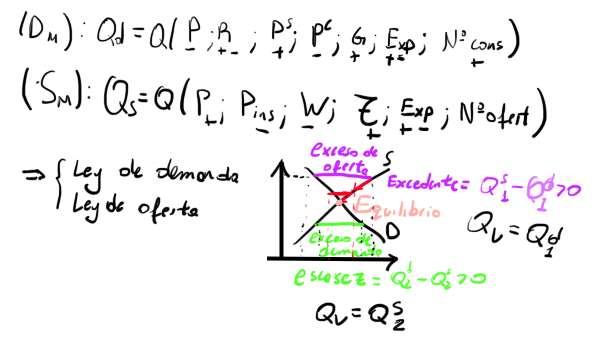
\includegraphics[width=8cm]{../Assets/ley_oferta_demanda.png}

\chapter{Macroeconomia}

\section{Posibles definiciones}

\begin{enumerate}
	\item \textbf{Sachs y Larraín}: Estudia el crecimiento y las fluctuaciones de la economía de país desde una perspectiva amplia.
	\item \textbf{Abel y Bernake}: Es el estudio de las estructuras y los resultados de las economías nacionales y de las medidas que emplean los gobiernos.
	\item \textbf{Gregory y Mankiw}: Es el estudio de los fenómenos que afectan al conjunto de la economía como la \textbf{inflación}, el \textbf{desempleo} y el \textbf{crecimiento económico}.
\end{enumerate}

\section{Inflacion}
\textbf{Definición}: Es el aumento sostenido y generalizado de los precios. \\

Definiremos el \(ISP\) como:
\[\boxed{ISP_i^{(0;t)}= \frac{P_i^t}{P_i^0} \cdot 100}\]
donde \(i\) es un bien o servicio, \((0;t)\) es el periodo de tiempo entre \(0\) (momento base) y \(t\) (momento actual), \(P_i^0\) es el precio del bien \(i\) en el momento base y \(P_i^t\) es el precio del bien \(i\) en el momento actual. \\

Es facil concluir que:
\[ISP_i^{(0;0)}= \frac{P_i^0}{P_i^0} \cdot 100=100\]


Podemos definir una matriz \(\{ g \}^{i=1,...,n}_{j=1,...,m}\)
donde $j$ es una familia muestra. \\

La suma de todos los elementos de la matriz:
\[
	G=
	\sum_{i=1}^{n}{\sum_{j=1}^m{{g_{ij}}}}
\]

Definimos:
\[
	w_i^0=
	\frac{g_i}{G}
\]

y se cumple:
\[
	\sum_{i=1}^{n}{w_i^0}=
	\sum_{i=1}^{n}{\frac{g_i}{G}}=
	\frac{\sum_{i=1}^{n}{g_i}}{G}=
	\frac{G}{G}
	=1
\]

\subsection{IPC}
Ahora podemos definir el \(IPC\), el Indice de Precios de Consumo.

\[
	\begin{array}{rl}
		IPC^{(0;t)}
		 & = \sum_{i=1}^{n}{ISP_i^t \cdot w_i^0}                                   \\
		 & = \sum_{i=1}^{n}{\frac{P_i^t}{P_i^o} \cdot w_i^0 \cdot 100}             \\
		 & = \sum_{i=1}^{n}{\frac{P_i^t \cdot q_i^0}{P_i^0 \cdot q_i^0} \cdot 100}
	\end{array}
\]
La ultima formula se le llama IPLaspeyres

\subsection{Caracteristicas}
\begin{enumerate}
	\item Canasta fija
	\item Cantidad fija
	\item Ponderacion fija
\end{enumerate}

\subsection{Criticas}
\begin{enumerate}
	\item Los bienes pueden cambiar a lo largo del tiempo. Hay bienes que desaparecen sin tener sustitutos o bienes que son nuevos pero que no esta capturado en el indice.
	\item La importancia que tiene cada bien puede ir cambiando a medida que pasa el tiempo.
\end{enumerate}

\subsection{Otras cosas}

\(IPC^{(0;0)} = 100\)

\subsection{Variacion del IPC}

Si tenemos tres momentos en el tiempo (el base "0", el "t"\ y el "h")

\(\text{Variacion absoluta}(t;h) = IPC^h - IPC^t\) \\

\(\text{Variacion relativa}(t;h) = \frac{IPC^h - IPC^t}{IPC^t} =
\frac{IPC^t}{IPC^h} -1\) \

\(
\text{Variacion porcentual}(t;h) =
\frac{IPC^h - IPC^t}{IPC^t} \cdot 100 =
(\frac{IPC^t}{IPC^h} -1) \cdot 100
\) \\

Se suele llamar a la variacion porcentual $\pi$ \\

Observar:
\[
	\pi (0;t) = (\frac{IPC^t}{IPC^0} - 1) \cdot 100
	= (\frac{IPC^t }{100} - 1) \cdot 100
	= \frac{IPC^t\cdot 100}{100} - 100
	= IPC^t - 100
\]
\[
	\Rightarrow
	\boxed{
		\pi (0;t) = IPC^t - 100
	}
\]

\noindent\fbox{
	\parbox{\textwidth}{
		CUIDADO: esto no se cumple para porcentajes que no son el 0. Porcentajes que se acumulan no se suman.
	}
} \\

Tenemos: \( \pi (t;h) \) y \( \pi (h;k) \) \\

Queremos:
\( \pi (t;k) \)

\[
	\pi (t;h) = (\frac{IPC^h}{IPC^t} - 1) \cdot 100
	\Rightarrow
	\frac{IPC^h}{IPC^t} = \frac{\pi (t;h)}{100} + 1
\]
\[
	\pi (h;k) = (\frac{IPC^k}{IPC^h} - 1) \cdot 100
	\Rightarrow
	\frac{IPC^k}{IPC^h} = \frac{\pi (h;k)}{100} + 1
\]

\[
	\pi (t;k) = (\frac{IPC^t}{IPC^k} - 1) \cdot 100
	= (\frac{IPC^t \cdot IPC^h}{IPC^k \cdot IPC^h} - 1) \cdot 100
	= (\frac{\frac{IPC^h}{IPC^k}}{\frac{IPC^h}{IPC^t}}  - 1) \cdot 100 \\
	= (\frac{\frac{\pi(h;k)}{100} + 1}{\frac{\pi(t;h)}{100} + 1} - 1) \cdot 100
\]

De manera general:
\[
	\boxed{
		\pi^{\text{anual}} =
			[\prod^{12}_{i=1} (1 + \frac{\pi^i}{100}) - 1 ] \cdot 100
	}
\]

Y el valor promedio para un mes:
\[
	\boxed{
		\overline{\pi} = ( \sqrt[n]{1 + \frac{\pi^{\text{anual}}}{100}} - 1) \cdot 100
	}
\]
con $n$ siendo las particiones del periodo anual.

\section{PIB}
El PIB es: valor de bienes y servicions finales generados en una economia, en un periodo determinado (normalmente 1 año) \\
\subsection{PIB nominal}
$PIB_{nominal}^t = \sum_{i}{p_i^t q_i^t} = P^t Q^t$ \\

$PIB_{nominal}^{t-1} = P^{t-1}Q^{t-1}$ \\

\(\left.
	\begin{array}{l}
		\text{Variacion}[(t-1);t] = (\frac{PIB_N^t}{PIB_N^{t-1}} - 1) \cdot 100 \\
		Supuestos: \begin{array}{l}           \\
			           Q^{t-1}=Q^t=Q \\
			           P^t > P^{t-1} \\
		           \end{array}
	\end{array}
	\right\} \Rightarrow \begin{array}{l}
		(\frac{P^tQ^t}{P^{t-1}Q^t} - 1)\cdot 100 = \\
		(\frac{P^t}{P^{t-1}} - 1) \cdot 100 > 0
	\end{array}\) \\

PIB nominal no sirve para medir crecimiento, es distorcionado por inflacion

\subsection{PIB real}

$PIB_R = \overline{PIB}_{t-1}^t = P^{t-1}Q^t$ \\

$\overline{PIB}_{t-1}^{t-1} = PIB_N^{t-1} = P^{t-1}Q^{t-1}$ \\

$\left.
	\begin{array}{l}
		\text{Variacion}[(t-1);t] = (\frac{PIB_R^t}{PIB_R^{t-1}} - 1) \cdot 100 \\
		Supuestos: \begin{array}{l}           \\
			           Q^{t-1} > Q^t \\
			           P^t = P^{t-1} \\
		           \end{array}
	\end{array}
	\right\} \Rightarrow \begin{array}{l}
		(\frac{P^{t-1}Q^t}{P^{t-1}Q^{t-1}} - 1)\cdot 100 = \\
		(\frac{Q^t}{Q^{t-1}} - 1) \cdot 100 > 0
	\end{array}$ \\

\subsection{IPI}

$IPI = \frac{PIB_N^t}{PIB_R^t}\cdot 100 = \frac{P^tQ^t}{P^0Q^t} \cdot 100 = \frac{P^t}{P^0} \cdot 100$

\subsection{PBN}

\[
	PBN = PIB + \underbrace{PNF}_{*} \\
\]
\[
	* = [\text{Ingreso residentes en el exterior - ingreso de los \textbf{no} residentes en la economia}]
\]


\subsection{VBP (Valor Bruto de Produccion)}
\[
	VBP = VII + VAB
\]
donde: $VII$ es Valor de los Insumos Intermedios y $VAB$ es el Valor Agregado Bruto \\
Ademas: \[
	VAB = PIB
\]

Agentes economicos =
\[
	\left\{\begin{array}{ll}
		Familias                          & \rightarrow Consumo (C)                         \\
		Empresas                          & \rightarrow \text{Inversion Privada} (I_{PR})   \\
		Gobierno                          & \rightarrow \text{Inversion del Gobierno} (I_g) \\
		                                  & \rightarrow \text{Consumo del Gobierno} (G)     \\
		\text{Sector Externo} \rightarrow &
		\left\{ \begin{array}{l}
			        Venta \rightarrow Exportaciones (X) \\
			        Compras \rightarrow Importaciones (M)
		        \end{array}\right.
	\end{array}\right.
\]

\( I_{PR}+I_g = I \) \\
\[
	PIB = C + I_{PR} + I_g + G + X - M
\]


\end{document}
